\section{Methodology}

The proposed study follows a computational approach based on a continuum description of the coupled electromechanical system. 
The methodology is structured in several stages, combining physical modeling with numerical approximation.

First, the governing equations of elasticity and electrical conduction are formulated within a consistent continuum framework. 
The mechanical problem provides the displacement field $u$, from which the strain tensor $\varepsilon(u)$ is computed. 
This strain field enters the electrical problem through the strain-dependent conductivity $\sigma(\varepsilon)$.

As a baseline, the electrical conduction problem with constant conductivity is considered and solved numerically. 
This case admits an analytical solution and serves to validate the numerical implementation. 
A finite element discretization is employed, and the numerical solution is compared against the exact solution to ensure correctness.

\begin{figure}[htbp]
    \centering
    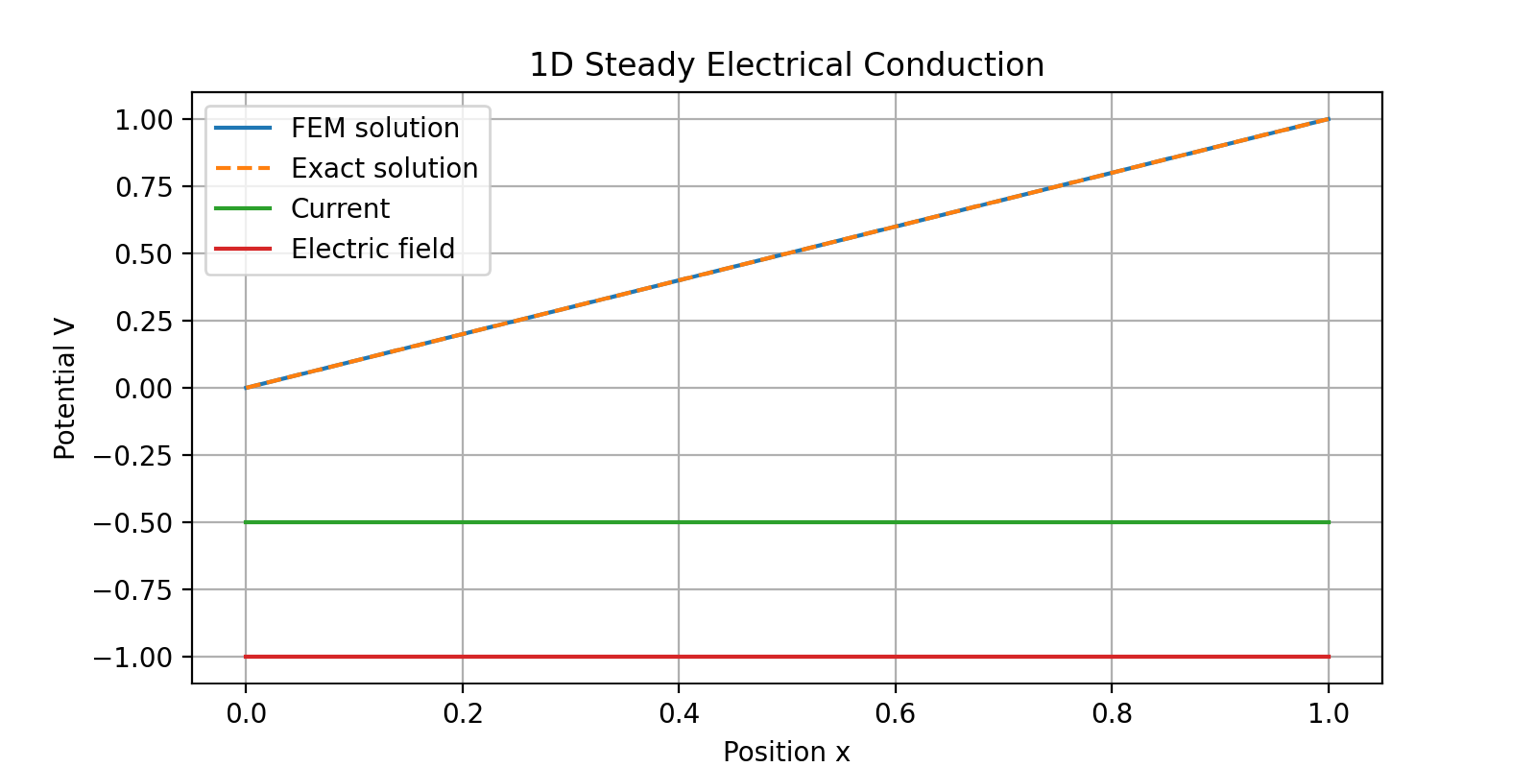
\includegraphics[width=0.75\textwidth]{Images/1d_cond.png}
    \caption{Finite element solution of the 1D steady conduction problem with constant conductivity compared with the analytical solution. 
    The linear potential profile and constant electric field confirm the expected physical behavior.}
\end{figure}

This baseline case also provides a reference for interpreting deviations introduced by strain-dependent conductivity in the coupled problem.

Building on this, the full coupled system is addressed by introducing a spatially varying conductivity $\sigma(\varepsilon(u))$. 
The problem is solved iteratively: starting from an initial displacement field, the strain is computed, the conductivity is updated, 
and the electrical problem is solved. This procedure is repeated until convergence is achieved.

The resulting system is nonlinear due to the dependence of $\sigma$ on $\varepsilon(u)$, and particular attention is given to the stability 
and convergence of the numerical scheme, as well as to the sensitivity of the solution with respect to deformation.

From a computational perspective, the finite element method (FEM) is used as the primary discretization technique due to its flexibility 
in handling heterogeneous material properties and complex geometries. The implementation emphasizes clarity and modularity, allowing 
systematic exploration of different forms of the strain–conductivity relation.

Beyond purely phenomenological models, the framework is designed to accommodate physically motivated constitutive relations. 
In particular, the function $\sigma(\varepsilon)$ can be informed by transport models derived from electronic structure calculations, 
or approximated using data-driven approaches when such data is available.

Overall, the methodology provides a transparent and extensible computational pipeline that connects continuum modeling 
with physically grounded descriptions of strain-dependent conductivity.